\documentclass[tikz,border=6pt]{standalone}
\usepackage{amsmath,amssymb}
\usepackage{xcolor}
\definecolor{accent}{HTML}{A13D2C}
\definecolor{accent2}{HTML}{2B5F6B}
\definecolor{muted}{HTML}{5A564F}
\definecolor{panel}{HTML}{F8F6F0}
\definecolor{linecol}{HTML}{D8D2C4}
\definecolor{astroblue}{HTML}{1B4F72}
\definecolor{ink}{HTML}{1E1C1A}
\usetikzlibrary{calc,arrows.meta}
\usepackage[T1]{fontenc}\usepackage{newpxtext,newpxmath}  % same fonts as the notes
\begin{document}
% Stellar populations as a tree: stars split first by whether their birth gas held any metals (Z = 0 or not),
% then by how much. Each leaf gives age, metal fraction Z, where the stars live and examples from this chapter.
% The arrow along the bottom is the order in which the populations formed, as each generation enriched the gas.
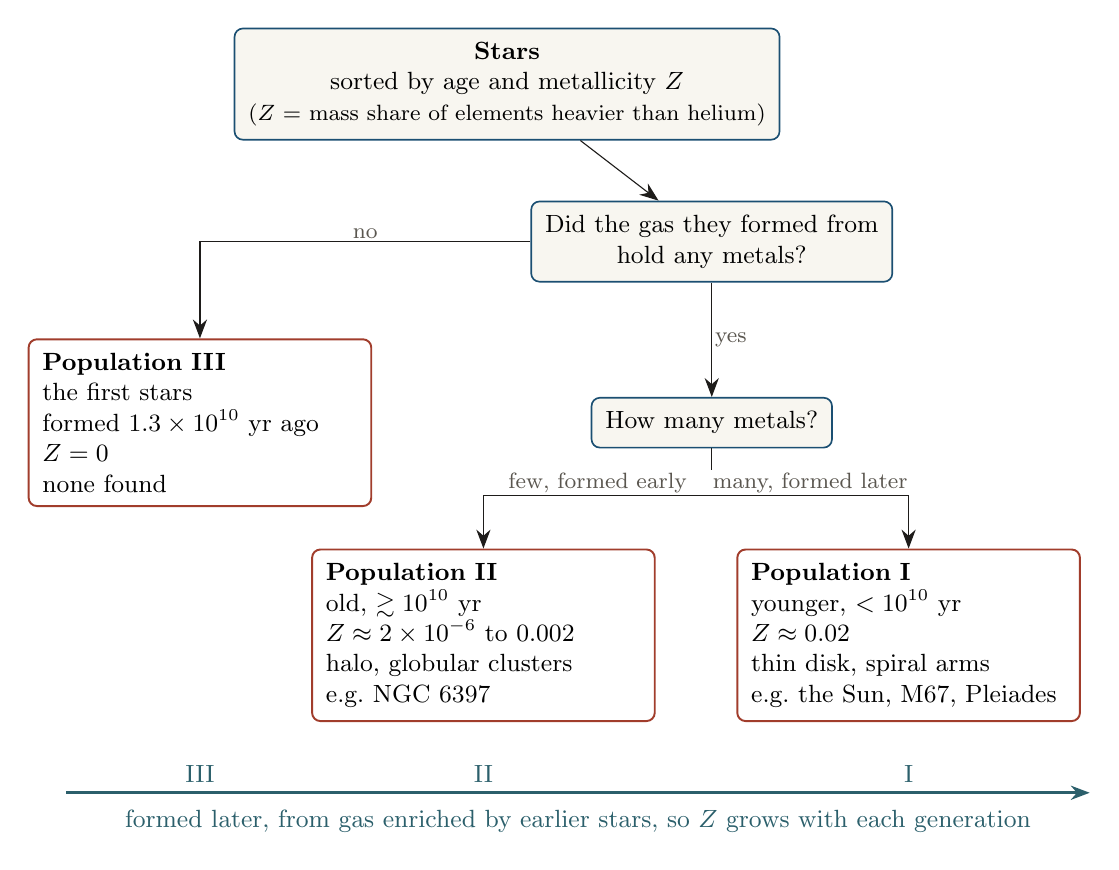
\begin{tikzpicture}[font=\small, >={Stealth[length=2.4mm]},
  q/.style={draw=astroblue, line width=0.6pt, fill=panel, rounded corners=3pt, align=center, inner sep=5pt},
  leaf/.style={draw=accent, line width=0.7pt, fill=white, rounded corners=3pt, align=left, text width=4.0cm, inner sep=5pt},
  lab/.style={muted, font=\footnotesize, fill=white, inner sep=1pt}]
  \node[q] (root) at (0,0) {\textbf{Stars}\\ sorted by age and metallicity $Z$\\ \footnotesize($Z$ = mass share of elements heavier than helium)};
  \node[q] (q1) at (2.6,-2.0) {Did the gas they formed from\\ hold any metals?};
  \node[leaf] (p3) at (-3.9,-4.3) {\textbf{Population III}\\ the first stars\\ formed $1.3\times10^{10}$ yr ago\\ $Z=0$\\ none found};
  \node[q] (q2) at (2.6,-4.3) {How many metals?};
  \node[leaf] (p2) at (-0.3,-7.0) {\textbf{Population II}\\ old, $\gtrsim10^{10}$ yr\\ $Z\approx2\times10^{-6}$ to $0.002$\\ halo, globular clusters\\ e.g.\ NGC~6397};
  \node[leaf] (p1) at (5.1,-7.0) {\textbf{Population I}\\ younger, $<10^{10}$ yr\\ $Z\approx0.02$\\ thin disk, spiral arms\\ e.g.\ the Sun, M67, Pleiades};
  \draw[ink, ->] (root) -- (q1);
  \draw[ink, ->] (q1.west) -| node[lab, pos=0.25, above] {no} (p3.north);
  \draw[ink, ->] (q1) -- node[lab, right] {yes} (q2);
  \draw[ink, ->] (q2.south) -- ++(0,-0.6) -| node[lab, pos=0.25, above] {few, formed early} (p2.north);
  \draw[ink, ->] (q2.south) -- ++(0,-0.6) -| node[lab, pos=0.25, above] {many, formed later} (p1.north);
  % time arrow
  \draw[accent2, ->, line width=1pt] (-5.6,-9.0) -- (7.4,-9.0);
  \node[accent2, anchor=north, align=center] at (0.9,-9.1) {formed later, from gas enriched by earlier stars, so $Z$ grows with each generation};
  \node[accent2, anchor=south] at (-3.9,-9.0) {III};
  \node[accent2, anchor=south] at (-0.3,-9.0) {II};
  \node[accent2, anchor=south] at (5.1,-9.0) {I};
\end{tikzpicture}
\end{document}
